% !TeX spellcheck = en_US
\section{Real-Time Video Quality Calculation}
\label{sec:723_QualityCalculation}
\ac{VAS} aims for supporting streaming sessions in adapting according to the perceived quality of the different representations of a \ac{DASH} session.
To determine the perceived quality of different video representations an objective \ac{FR} quality algorithm is used.
Besides a reliable prediction of the perceived quality a short algorithm run-time is favored to support for live streaming or video conferencing scenarios.
None of the existing algorithms combines a reliable quality prediction and fast algorithm execution.
Therefore, two algorithms are selected to illustrate that \ac{VAS} can even support upcoming developments in the perceived quality estimation.
%This section describes the \ac{SUQA} an improved quality assessment algorithm relying on leveraging \ac{GPU}s for fast execution.
%\subsection{Usage of VQM}

The \ac{VQM} algorithm by Pinson et al.~\cite{Pinson2004} has been selected to be the basis of our \ac{RT-VQM} component in \ac{VAS}.
The essential steps of \ac{VQM} are depicted in Figure~\ref{fig:720_vqmsteps}, which depicts the steps of the \ac{VQM} calculation as described in Section~\ref{label}.
\begin{figure}[t]
	\centering
	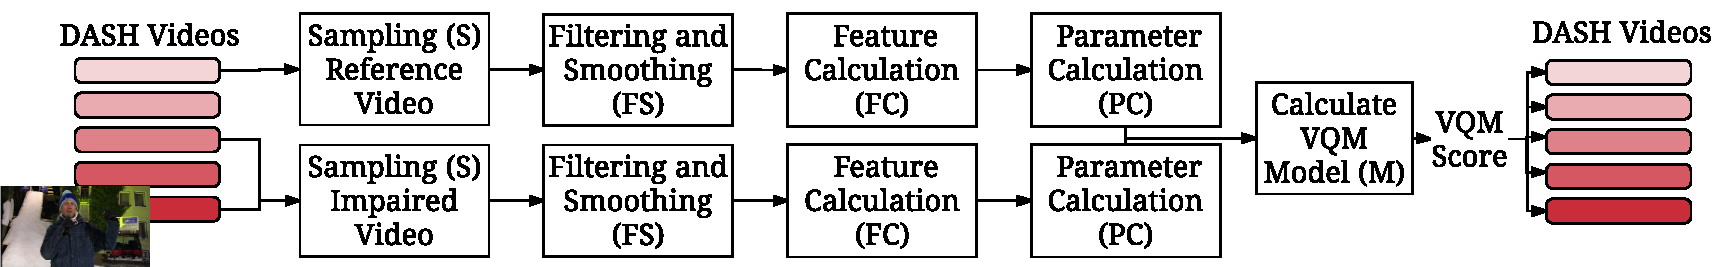
\includegraphics[width=\textwidth]{./gfx/700_VAS/VQMDash}
	\caption{Essential steps of a VQM measurement between a reference representation and other DASH representations (inspired by Pinson et al.~\cite{Pinson2004}).}
	\label{fig:720_vqmsteps}
\end{figure}
In contrast to the discussion in the background, the quality of each \ac{DASH} representation in relation to the highest bit rate representation is assessed.
An algorithm execution starts with a selection of two different \ac{DASH} representations --- a reference and an representation to be assessed.
The highest bit rate representation acts as a reference to determine the perceived quality of the other lower bit rate representations.
Remaining steps in this approach are similar to the discussion before.
As a FR method \ac{VQM} can only determine the quality of each representation in relation to one reference representation, the \ac{VQM} calculation is conducted for all representations in relation to the highest \ac{DASH} representation.

The quality assessment is repeated for each representation of a video and quality values are calculated for individual video shots. 
%The representations need to be decoded into the YCbCr color space, which contains one luma channel (Y) and two chrominance channels (CbCr).
%The first step contains is called the \acf{S} of the two video representations --- the reference and assessment representation. 
%\ac{S} converts two time-aligned video frames into a floating point format, which provides the required accuracy for a precise estimation of the perceived quality.
%
%The task of the \emph{Calibration} is the synchronization of video frames between different video representations, which may become potentially desynchronized by the transmission over analogue transmission channels.
%This step is not necessary, when \ac{DASH} and the Internet is used.
%
%%Filtering
%The \acf{FS} applies the Sobel edge filter~\cite{Sobel1968} to the synchronized frames of the two video representations. 
%To analyze the changes of resolution or quantization differences between the reference and the assessment frame a edge difference metric is calculated, whereas temporal differences, e.g., by different frame rates, are determined in a temporal metric.
%This is done relying on visual features in the \acf{FC} step within the video frame (S) and across frames (T), which are combined in an \acf{ST-Region}.
%It pans across $8\times8$ pixels and $6$ frames at a frame rate of 30, i.e., 0.2 seconds of video.
%Five different feature-sets are extracted from the \ac{ST-Region} including two feature sets focus on structural information%(\emph{SI}, \emph{HV})
%, on color information %(\emph{COHER\_COLOR}), 
%on contrast %(\emph{CONT}), and one on
%and on motion (\emph{ATI}).
%The resulting \ac{ST-Region} from both representations are compared by the \ac{PC} step, resulting in an \ac{ST-Region} error matrix quantifying the differences between both videos.
%Afterwards the errors of each feature across the \ac{ST-Region}s are condensed into a single value and for different \ac{ST-Region} a linear regression model determines the resulting \ac{VQM} value in a \acf{M} step.
%Then a linear regression model is mapped to the \ac{ST-Region} values.
%The regression models has been validated in extensive subjective studies. 
%This \acf{M} step calculates the combined 
The \ac{VQM} values range from 0 --- reference and assessment representation are equal --- to 1 --- a significantly degraded video sequence.
Yet, for understanding which thresholds separate high from good and bad quality, a mapping is introduced to the well-researched \ac{MOS} concept.
This mapping has been studied by Zinner et al.~\cite{Zinner2010}.% and is used for \ac{SUQA}.

The \ac{VQM} implementation is not able to compare reference and test sequences in different resolutions and frame rates internally. 
Therefore, in a joint work a real-time quality assessment of \ac{VQM} has been developed, which allows scaling of videos by leveraging the execution on a \ac{GPU}.
This version is called RT-VQM~\cite{Wichtlhuber2016}, but not part of the discussion in the thesis.

%In addition, a more recent and more accurate video quality metric proposed by Netflix is used: \ac{VMAF} to show how versatile \ac{VAS} is.
%The correlation with subjective evalu of \ac{VMAF} is higher 
%This functionality has to be enhanced in the proposed implementation of the \ac{SUQA}.
%\subsection{Usage of VMAF}
%\subsection{Idea and Requirements}
%%Idea of RT_VQM - Parallelize code on cuda and improve the speed
%%Requirement: spatial, quantization and frame rate impact
%%Requirement: Improved speed, but the same precision
%%Requirement: Mapping to a general quality metric which can easily be mapped to other metrics
%The central idea of the \ac{SUQA} component is the acceleration of a reliable perceived quality assessment by massive parallelization.
%The parallelization of the quality assessment promises significant speed-ups as existing algorithms rely on a limited number of feature detection and analysis steps repeated for a large number of pixel blocks in a many video frames. 
%To realize such a parallelization, we design \ac{SUQA} to be run on \ac{GPU}s. %, whereas they are classically run on \ac{CPU}s.
%Whereas a \ac{CPU} is designed for general purpose calculations, the design of a \ac{GPU} is optimized for visual, image and video processing
%In addition, the number of processing cores is by an order of magnitude higher compared to a \ac{CPU}.
%The different designs of \ac{CPU} and \ac{GPU} require to re-design central elements to allow an efficient parallelization of the quality assessment.
%
%Besides a significant run-time decrease, we postulate three requirements that the new algorithm needs to fulfill.
%
%The first requirement addresses, that the algorithm should be capable to analyze differences in all of the three dimension a video can be encoded: the spatial (resolution), the temporal (frame rate) and the quality dimension (\ac{SNR}).
%As \ac{DASH} representations can be encoded being different in all three dimensions, \ac{VAS} and thus \ac{SUQA} must be able to detect these changes, too.
%
%The second requirement addresses, that our main goal is to accelerate an existing algorithm, but without any perceivable loss of precision. 
%The quality estimation of \ac{SUQA} shall be similar to the one of non-accelerated algorithm.
%
%A last requirement is the mapping of the algorithm results to the models known for perceived video quality research.
%A well-known model is the \ac{MOS}~\ref{ITU-J800}, which depicts the perceived quality in a range from 1 (worst quality) to 5 (best quality)~\cite{Seufert2015}.
%The resulting \ac{VQM} value spans between 0 (best quality) and 1 (worst quality) and can be mapped to the \ac{MOS} model using the approach of Zinner et al.~\cite{Zinner2010}, which formulates a simple decreasing linear function between \ac{VQM} values and the \ac{MOS}.
%% ------------------------------
%% This helps to  prepare different quality models for different device configurations, e.g. the quality model for a mobile device capable for Full HD resolution is different from a device solely capable for 360p resolution.
% %==========================================================================================================================================================
% %==========================================================================================================================================================
%\subsection{Analysis for Run-time Improvement Potential}
%The speed-up of \ac{SUQA} in comparison to \ac{VQM} shall be achieved by improving the most promising steps of the algorithm.
%Therefore, the potential for improvement of each step in \ac{VQM} shall be assessed.
%\subsubsection{Metrics for Analysis}
%Three measures are used to analyze \ac{VQM}, namely the \emph{throughput} $T$, the \emph{arithmetic intensity} $A$ and the \emph{execution time} $E$ of each step.
%
%The throughput ($T$) represents the absolute number of pixels which can be analyzed in a given time period, e.g., a second.
%It is defined as:
%\begin{equation}
%\unitfrac[T]{MPixel}{s} = \frac{r_h * r_v * |f|}{t},
%\end{equation}
%where $r_h$ and $r_v$ are the horizontal and vertical resolution of each video frame, $|f|$ represents the number of frames and $t$ is the length of the assessed video segment. 
%Intuitively, $T$ measures the number of pixels of a video sequence that can be processed per second. 
%It determines how many video representations can be processed in parallel by the algorithm, so if the sum of pixels of all video representations that are processed per second is lower than $T$ - the algorithms allows in real-time processing of the \ac{DASH} video.
%$T$ is a well suited measure for identifying bottleneck processing steps worth to be accelerated. 
%
%Yet, $T$ is not suitable to determine, if the steps are suitability for parallelization, which can be determined using the arithmetic intensity ($A$).
%It is defined as:
%\begin{equation}
%\unitfrac[A]{FLOP}{LDST} = \frac{\unit[C]{FLOP}}{\unit[M]{LDST}},
%\end{equation}
%where $C$ represents the number of \acp{FLOP} and $M$ is the number memory access operations called \ac{LDST}.
%A high arithmetic intensity identifies steps bound by processing capabilities and not bound by \ac{I/O} operations, which makes them especially suitable for a parallelization using \acp{GPU} \cite{NVIDIA2014a}.
%
%The execution time $P$ shows in comparison to the total run time of the algorithm the fraction of processing time that can be accounted to this step.  
%%==========================================================================================================================================================
%%==========================================================================================================================================================
%\subsubsection{Results of the Analysis}
%We performed an analysis on different versions of videos from the LIVE Mobile video database using $15\unit{s}$ of video at 30 $\unit{FPS}$ for three different resolutions from WSIF ($680\times384$), over WVGA ($720\times400$) to 720p ($1280\times720$).
%The results illustrated in Figure~\ref{fig:stepwiseref} consists of the assessment repeated 10 times without any significant deviation.
%\begin{figure}[t!]
%	\centering    
%		\subfloat[][]{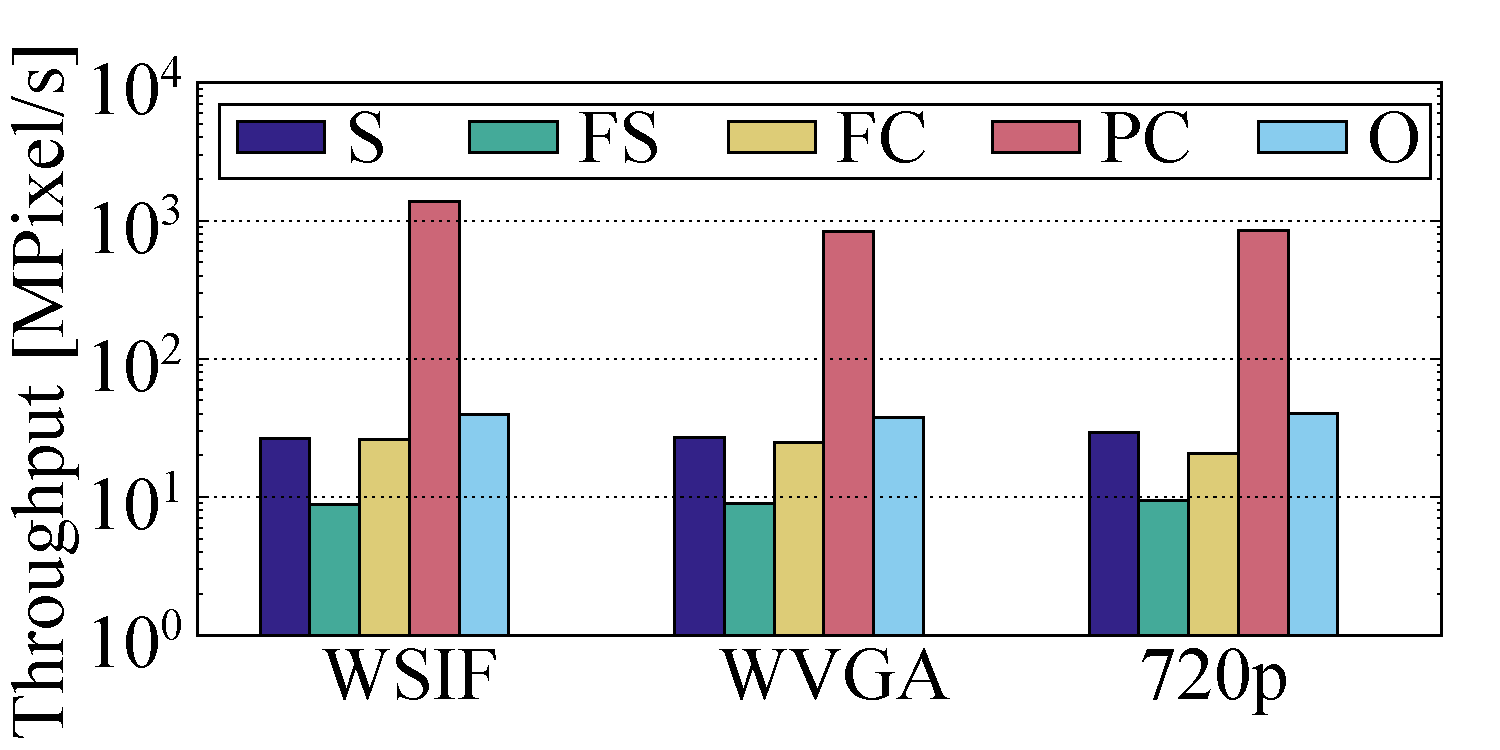
\includegraphics[width=0.32\columnwidth]{gfx/700_VAS/cpu_throughput}}
%		%\caption{Metric $T$ measured for different resolutions at 30 fps. The Other (O) category shows a code fraction, which could not be assigned to one of the categories.}
%		\subfloat[][]{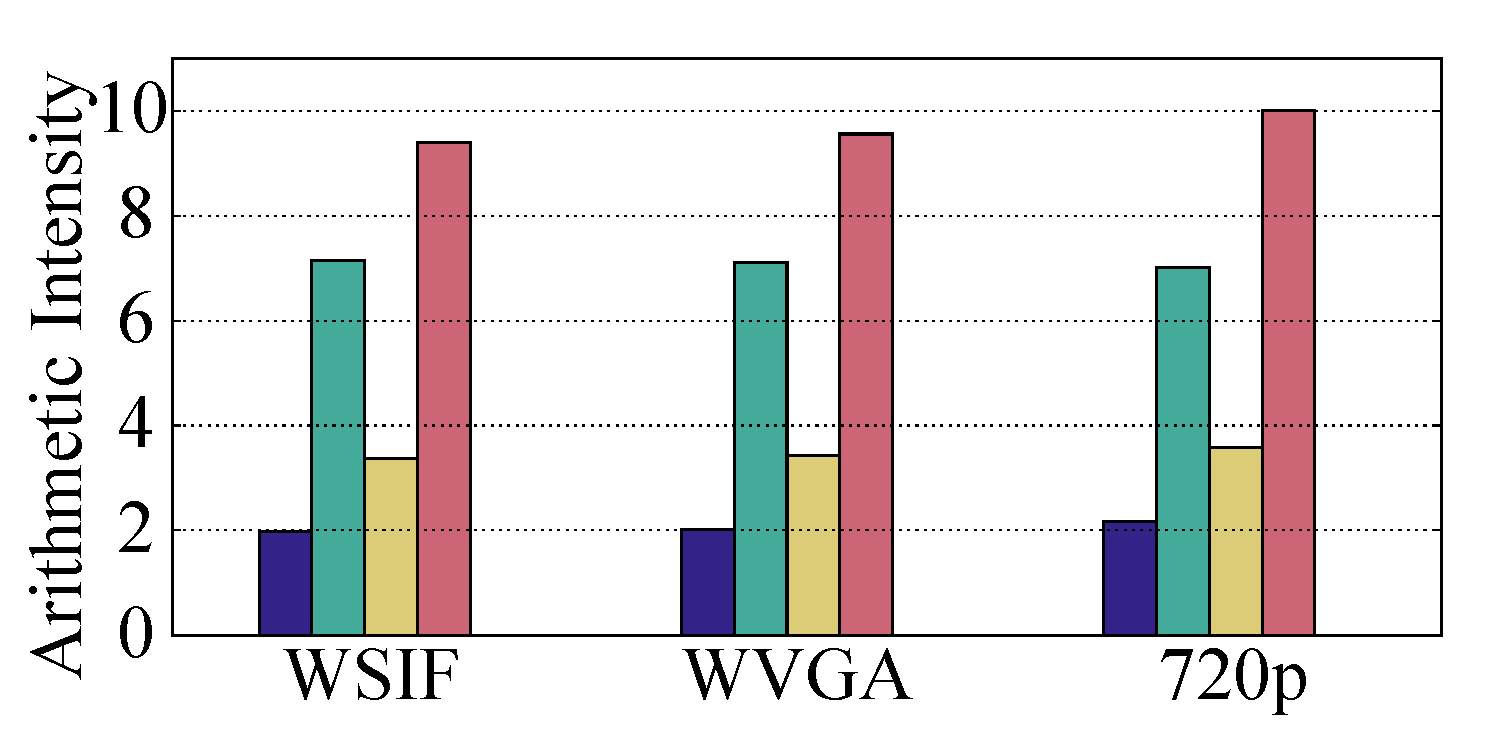
\includegraphics[width=0.32\columnwidth]{gfx/700_VAS/cpu_arithmetic_intensity}}
%		%\caption{Metric $A$, where only the Level 1 cache misses of the memory are considered.}
%		\subfloat[][]{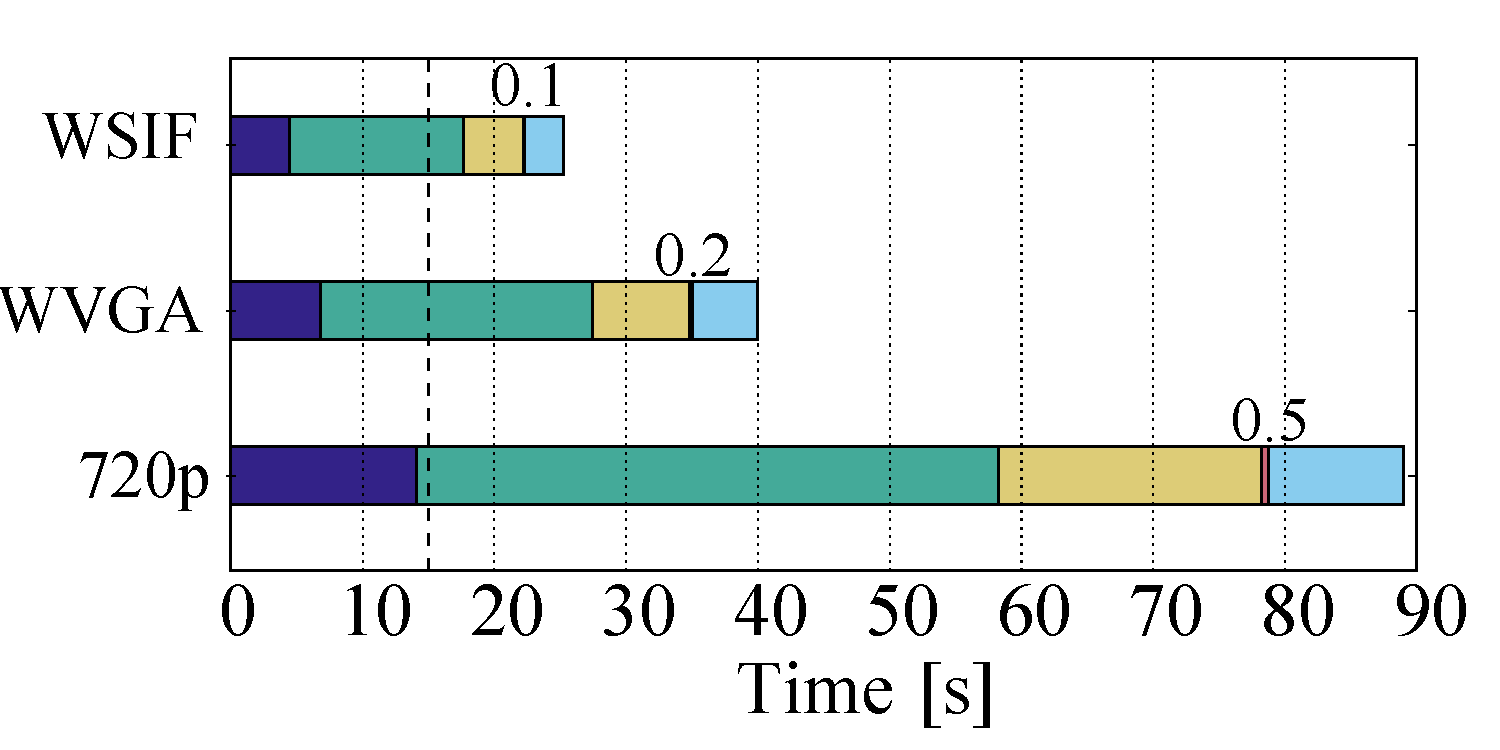
\includegraphics[width=0.32\columnwidth]{gfx/700_VAS/cpu_runtime}}
%		%\caption{Metric $E$, where the dashed line represents the execution time which would be necessary for real-time calculation.}
%		
%	\caption{Metrics for assessing the possibility to parallelize \ac{VQM} for each calculation step. Depicted numbers represent the averages for $10$ runs of a $15\unit{s}$ video sequence from the LIVE Mobile database~\cite{Moorthy2012} at $30\unit{fps}$.}
%	\label{fig:stepwiseref}
%\end{figure}
%
%Major bottlenecks, as depicted in Fig.~\ref{fig:stepwiseref} (left), in terms of $T$ can be observed in the algorithm steps: \ac{S}, \ac{FS}, and \ac{FC}.
%What furthermore increases the processing time of the algorithm is a large proportion of copy operations, which cannot be clearly assigned to any of the algorithm steps (category \ac{O}). 
%\ac{VQM}'s \ac{PC} step shows the highest throughput in combination with a negligible execution time.
%It should be noted, that \ac{PC}'s throughput is nearly constant for all three resolutions.
%This indicates, that the performance of \ac{PC} scales linearly with the number of pixels to be processed.
%
%Figure~\ref{fig:stepwiseref} (b) illustrates the results of the calculation of the arithmetic intensity per \ac{VQM} step.
%%In order to account for the caching capabilities of modern \ac{CPU} hardware, 
%It measures the Level 1 cache misses, so memory access operations \ac{LDST} which need to be answered by the memory as the hardware cache lacks the data.
%The \ac{PC} step, which has shown the highest $T$ also shows the highest $A$.
%Yet, with a fraction of only 1\% of the total run-time, \ac{PC} has no major influence in achieving a significant speed-up.
%The \ac{FS} and \ac{FC} steps show high arithmetic intensities which makes them ideal candidates to be run on \ac{GPU}s in order to leverage massive parallelization.
%The \ac{S} has no significant potential to benefit from running it in parallel.
%%==========================================================================================================================================================
%%==========================================================================================================================================================
%\subsection{Design of the Speeded-up Quality Assessment}
%Based on the analysis of different algorithm steps of the \ac{VQM} algorithm, the most promising ones are determined to be sourced into independently executable functions on a \ac{GPU}, which are called kernel functions.
% Those steps showing a high arithmetic intensity at a low throughput are most promising to benefit from a parallelization.
% In addition, the run-time fraction of the step should account for a large proportion to the total run-time of the algorithm.
% 
% \begin{figure}[t!]
% 	\centering
% 	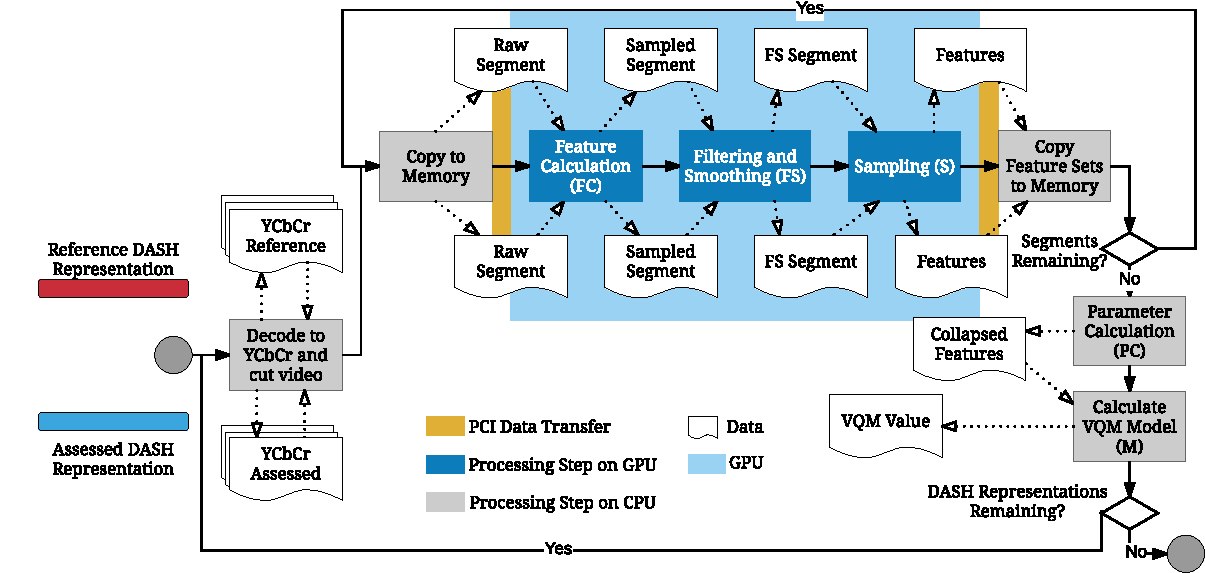
\includegraphics[width=0.98\textwidth]{./gfx/700_VAS/cuda_overview}
% 	\caption{Proposed \ac{VQM} calculation process on a \ac{GPU} system: The \ac{S}, \ac{FS} and \ac{FC} steps are performed on the \ac{GPU}}
% 	\label{figure:CUDA_overview}
% \end{figure}
%  
%From the previous analysis, we thus know that the \ac{S}, \ac{FS} and \ac{FC} steps are most promising for an acceleration on a \ac{GPU}
%Figure~\ref{figure:CUDA_overview} depicts the new algorithm used in the \ac{SUQA} component which will be discussed in more detail.
%At the same time, there is no promising potential for a parallelization of the \ac{PC} step.
%Consequently, \ac{SUQA} switches back to the \ac{CPU} for all following processing steps before executing the \ac{PC} step (see Figure~\ref{figure:CUDA_overview}).
% 
%For both, the reference representation and the assessment representation, the YCbCr formats are extracted and cut according to the required length, e.g., according to shot boundaries or \ac{DASH} segments (see Section~\ref{sec:721_shot_detection}). 
% The videos are transferred to the \ac{GPU} over the \ac{PCI} bus.
% On the \ac{GPU} the \ac{VQM} steps \acf{S}, \acf{FS} and \acf{FC} are executed and massively parallelized.
% On the \ac{CPU} the quality parameter calculation (PC) and the application of the regression model (M) for the final score calculation of the perceived quality are processed. 
% Both the \ac{PC} as well as \ac{M} show in the measurements of the standard implementation that they are insignificant in comparison to \ac{S}, \ac{FS} and \ac{FC}. 
% They are not considered for parallelization on a \ac{GPU}.
%%==========================================================================================================================================================
%%==========================================================================================================================================================
%\subsubsection{Sampling (S)}
%For the re-design of the \ac{S} step on a \ac{GPU}, it is important to understand, that \ac{GPU} and \ac{CPU} act as independent processing units.
%This means, that data to be processed on a \ac{GPU} needs to be transmitted over a \ac{PCI} bus, which can act as a bottleneck, if the data to be transferred is too large.
%\ac{S} is generating a large increase of data volume, as it transfers the video into a more verbose format by increasing the bit depth by a factor of 16.
%Thus, despite it in average low arithmetic complexity, we propose to conduct the \ac{S} step on the \ac{GPU} in order to reduce the data to be transferred over the \ac{PCI} bus.
%Furthermore, the transfer of data is coordinated by the proposed algorithm, so that slices of video can be transferred independently of each other to the \ac{GPU} and thus processed immediately.
%This reduces the startup latency of the assessment, as otherwise the complete video would be required on the \ac{GPU}.
%These asynchronous transfers achieve a nearly complete hiding of the \ac{PCI} bus latency. 
%The chunks to be transferred to the \ac{GPU} are determined by the size of the \ac{ST-Region}, i.e., six frames and $8\times8$ pixels.
%\subsubsection{\acf{FS}}
%The \ac{FS} step offers a huge potential for parallelization, as the arithmetic intensity is high at a low throughput.
%We run the different functions within this step to two different processes: the \emph{spatial} and \emph{temporal filtering}, and thus different kernel functions.
%Spatial filtering uses a Sobel filter~\cite{Sobel1968}, which runs a horizontal and an independent vertical filter operation relying on two multiplied convolution matrices $K=K_e \cdot K_s$. 
%Here, $K_e$ does the edge detection, whereas $K_s$ performs a smoothing of the edges. 
%$\cdot$ represents the matrix multiplication.
%\ac{SUQA} splits \acf{FS} to four \ac{GPU} kernel functions for the two edge operations and two smoothing filters. 
%Two as it is conducted, both, in the horizontal as well as the vertical direction of a video frame.
%The splitting of this functionality allows to run the calculations in the fast, but quick on-chip memory of the \ac{GPU}, whereas the full calculation in one run, would access the slow global memory.
%The temporal filtering is simple to be run on a \ac{GPU} as it calculates the luminance differences between consecutive frames.
% \subsubsection{\acf{FC}}
%The \ac{FC} step ensures that the results from the \ac{FS} step are pooled into a single feature value per \ac{ST-Region}.
%% The measurements of the reference implementation depicted in \autoref{fig:stepwiseref} indicate that the \ac{FC} step has a slightly higher throughput $T$ than the \ac{FS} step, however the arithmetic intensity is only roughly half as high.
%% This step is again a border case for parallelization.
%As the \ac{FC} step has a slightly higher throughput and only half the arithmetic complexity of the \ac{FS} step, the reason to perform it on the \ac{GPU} is caused by the impact of \ac{PCI} bus transfer times. 
%As the aim of this step is the combination of many intermediate results into a single value per \ac{ST-Region}, it is obvious that the transfer times after the \ac{FC} step will be significantly lower.
%During measurements it has shown, that the data to be transferred after the \ac{FC} step accounts for only around 3\% of the \ac{FS} data.
% 
%The main idea for improving the execution times in the \ac{FC} step is to design kernels for mean and standard deviation calculations which work quick in three dimensional data structures, as \ac{ST-Region} are analyzed.
%Yet, this is challenging, because the pooling often requires exclusive memory access and synchronization of in-parallel calculated threads.
%Thus, the aim is to ensure a high hardware utilization by constantly keeping threads executing calculations. 
%A challenge occurs, as for a pooling of one \ac{ST-Region} only a fixed number of threads can be assigned. 
%A too high number of threads paired with an according pooling design would cause threads to run out of work too early. 
%As the respective cores are bound to this calculation, this would waste resources until the complete calculation is completed.
%Figure~\ref{fig:pooling} shows that in our design four threads achieve a high and constant utilization of 87.5\%, which depicts the maximum within our analysis.
%
% \begin{figure}[t!]
% 	\centering    
% 	%\includegraphics[width=0.48\columnwidth]{./gfx/700_VAS/naive_pooling.eps}
% 	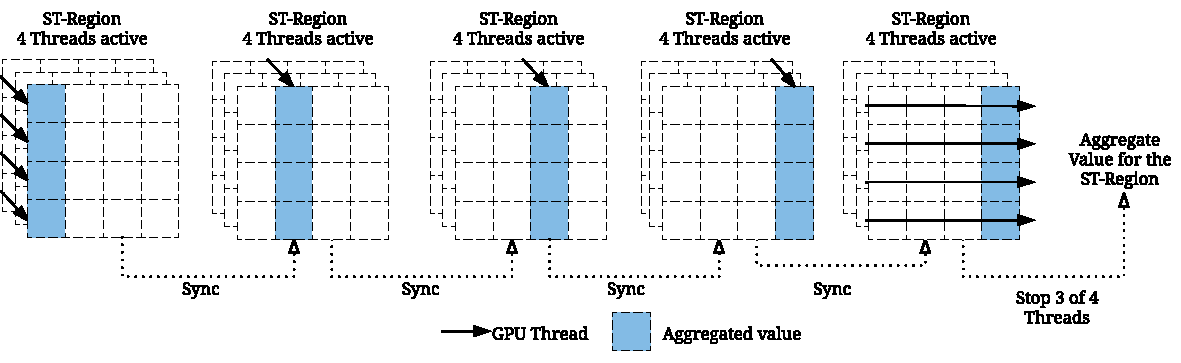
\includegraphics[width=0.98\columnwidth]{./gfx/700_VAS/optimized_pooling}
% 	\caption{Feature pooling strategy implemented for 4x4x4 \ac{ST-Region} using $4$ threads achieving a hardware utilization of 87.5\%.}
% 	\label{fig:pooling}
% \end{figure}
%Until the last step, which needs to be performed in a single thread, all threads are constantly processing calculations.
%The result is aggregated in the final step represents the input for the final quality calculation of \ac{VQM}.
%It contains six features sets aggregated for the whole video sequence that is analyzed.  
%Its data volume is small enough to be transferred back efficiently using the \ac{PCI} bus.
%% relying on standard \ac{VQM} calculations.
%\subsection{Speeded-up Scaling and Interpolation}
%One requirement for \ac{SUQA} is the capability to not only analyze different degradations induced by transmission errors, which cannot occur in \ac{DASH}, but compare different resolutions and frame rates. 
%This is not offered by the standard implementation of \ac{VQM}.
% 
%The interpolation between two resolutions is realized by representing the video sequence as a three dimensional texture.
%This allows to execute interpolation between different resolutions as fast as a \ac{GPU} can access its memory.
%From the video sequences the scaling can be done as the texture is represented as a continuous grid between the two resolutions.
%Similarly, different video frames can be represented in this grid, allowing frame rate conversions.
%Consequently, a fast spatial and temporal scaling to the reference video's resolution and frame rate is provided.
%%Whereas temporal linear interpolation between different frame rates requires additional calculations, the impact on the perceived quality is not clear.
%Another opportunity to reduce the run-time of \ac{SUQA} is thus to solely duplicate existing frames, when a lower frame rate representation needs to be scaled to a higher frame rate.
%By this, no new frames need to be sampled.
%%This mode has the advantage of being able to handle temporal downscaling even with frame rates other than $\frac{1}{2^n}, n \in \mathbb{N}$ of the reference video's frame rates.
%A further reduction in terms of run-time can be achieved by avoiding to re-run the \ac{S} step in \ac{SUQA} by not duplicating the frames, but only the already extracted features, which promises to be faster by an order of magnitude.
%This last method has been chosen in order to realize frame rate conversions.
%A condition of this method is that the two frame rates can be mapped to each other by a factor of $2^n$.
 %==========================================================================================================================================================
 %========================================================================================================================================================== 
\subsection{Integration into VAS}
 %Running on VAS server
 %Scalable by cloud services - AWS
 The integration of \ac{SUQA} into \ac{VAS} is realized as a cloud service achieving scalability by dynamically adding and removing \ac{GPU} instances.
 The central \ac{VAS} server acts as coordinator for assigning the calculations in a round robin manner to the available \ac{GPU} instances.
 As the computational complexity of the \ac{SUQA} component scales with the number of representations to be assessed and the resolution and frame rate of the reference representation, the estimation of the required \ac{GPU} instances is possible.
 
 A realization relies on the Amazon Web Service \ac{GPU} instance (g2.2xlarge)\footnote{NVIDIA GPU with 1536 cores and 15 GB memory}. 
 This realization was used during a live deployment~\cite{Wilk2016c} and is basis for the evaluation results in this chapter. 